\styledchapter[Proof of concept]{oplossing}
Om de PoC daadwerkelijk te maken moet er eerst gedefinieerd worden wat de scope is en hoe de PoC eruit gaat zien. De scope brengt in beeld wat er gedaan moet worden en wat de \acrfull{mvp} is. Op de \acrshort{mvp} kan de mock up gebaseerd worden. In dit hoofdstuk wordt de scope bepaald, delen van de mock up doorgelopen, uitleg gegeven over de PoC en kwaliteit van de code. Het hoofdstuk wordt afgesloten met een conclusie en advies

\section{User requirements verzamelen}\label{sec:ch7-user-requirements-verzamelen}
Om te begrijpen wat er gebouwd moet worden kunnen de behoeftes opgeschreven worden in de vorm van user stories. Een user story is de behoefte opgeschreven in een specifieke formaat om belangrijke informatie te achterhalen \cite{agile-user-story-template}. Een bekende formaat is de \textit{Connextra template} van Mike Cohn \cite{agile-user-story-template}: "\textbf{As a [role], I can [capability], so that [receive benefit]}". De template zorgt ervoor dat de rol (role), functie (capability) en reden (benefit) bekend is. In \autoref{fig:ch7-requirements} zijn alle user stories opgesteld, gegroepeerd in Epics. Bij elke user story is ook aangegeven of het \acrshort{mvp} is, welk prioriteit het heeft en de t-shirt size. De t-shirt size is een manier om op een hoog niveau aan te geven hoeveel werk een user story vereist. Een \textbf{S} vereist weinig werk terwijl \textbf{XL} veel werk vereist.

\begin{figure}[hbt!]
  \centering
  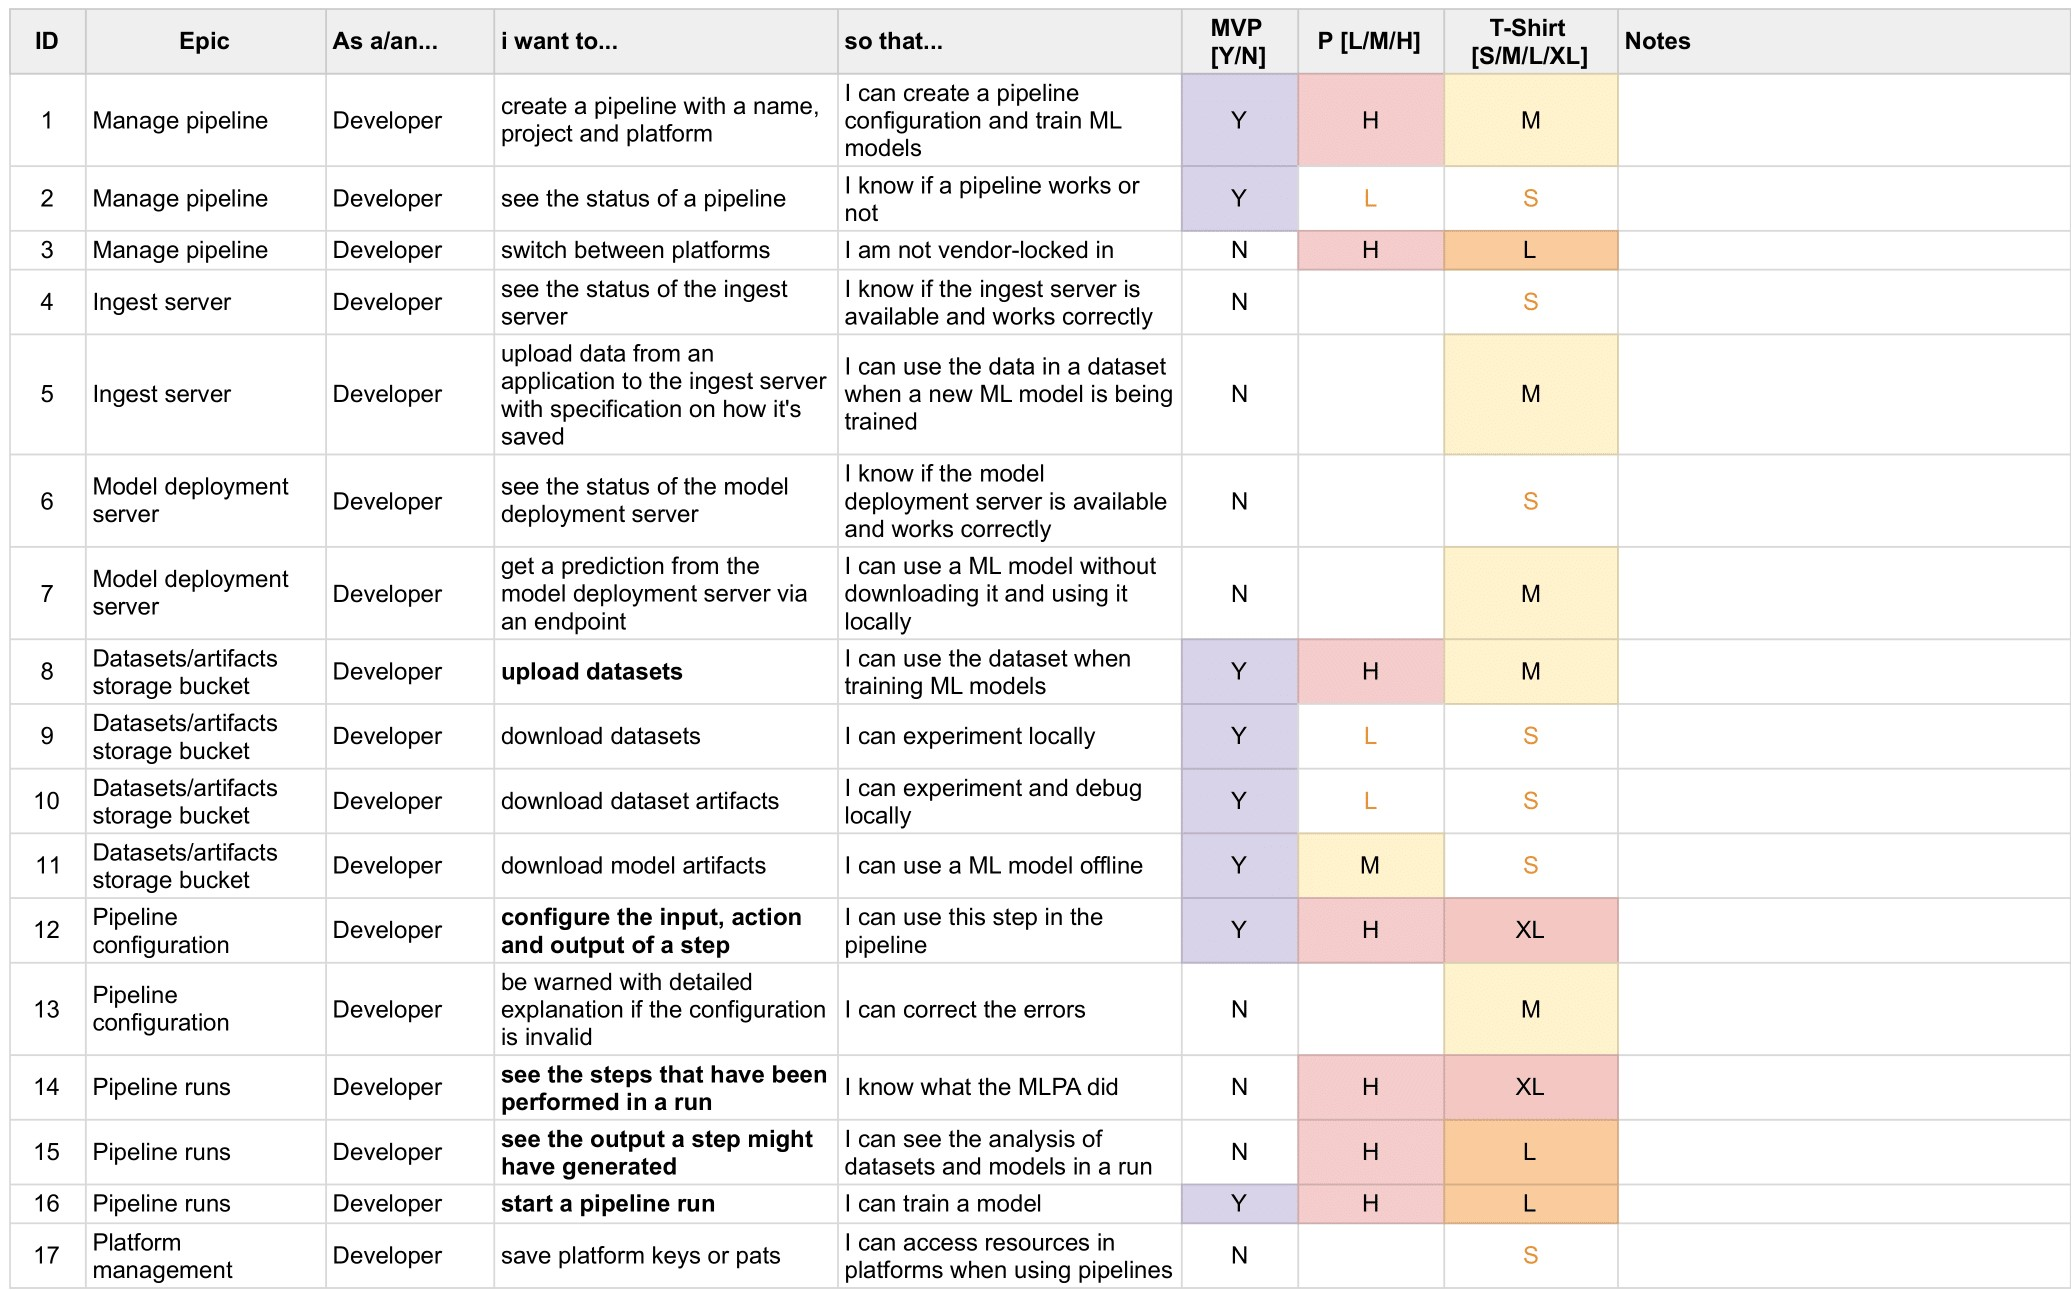
\includegraphics[width=1\textwidth]{chapter-7/requirements.jpg}
  \caption{Requirements opgesteld voor de proof of concept.}
  \label{fig:ch7-requirements}
\end{figure}

De user stories zijn opgesteld in samenwerking met de begeleiders van NGTI over het hele afstudeerproces. Nu de requirements zijn opgesteld, kan een Kanban bord opgericht worden om sprints te maken.

\newpage

\subsection{Requirements vertalen naar een scrum bord}\label{subsec:ch7-requirements-vertalen-naar-een-scrum-bord}
Een Kanban bord is een werkwijze om visueel aan te geven in welke stadia een taak is in het proces \cite{atlassian-kanban-board}. Taken in een Kanban bord vallen altijd onder een kolom om de status aan te geven. Een kolom kan bijvoorbeeld "todo", "doing", of "done"\space zijn. Een scrum bord is een vorm van een Kanban bord waarbij taken in een sprint zijn ingepland \cite{forecast-scrum-board}. Een sprint is een vaste periode van bijvoorbeeld een of twee weken waarin gewerkt wordt aan de ingeplande taken. Dit verschilt met een Kanban bord waarbij taken op elk moment toegevoegd kunnen worden. In software development kan dit niet; sprints zorgen ervoor dat er geen \gls{scope-creep} plaats vindt.

De user stories uit \autoref{fig:ch7-requirements} zijn vertaalt naar tickets in het scrum bord. Een user story is opgesplitst in meerdere tickets. Dit is het geval met bijvoorbeeld user story "upload datasets" (ID 8). Om deze functionaliteit te bouwen moet een storage bucket beschikbaar zijn en in de frontend de mogelijkheid zijn om dit te doen. In \autoref{fig:ch7-trello-w1-start} zijn de tickets aangemaakt met relevante labels om aan te geven bij welke epic een ticket hoort, of het \acrshort{mvp} is, de prioriteit en t-shirt size.

\begin{figure}[hbt!]
  \centering
  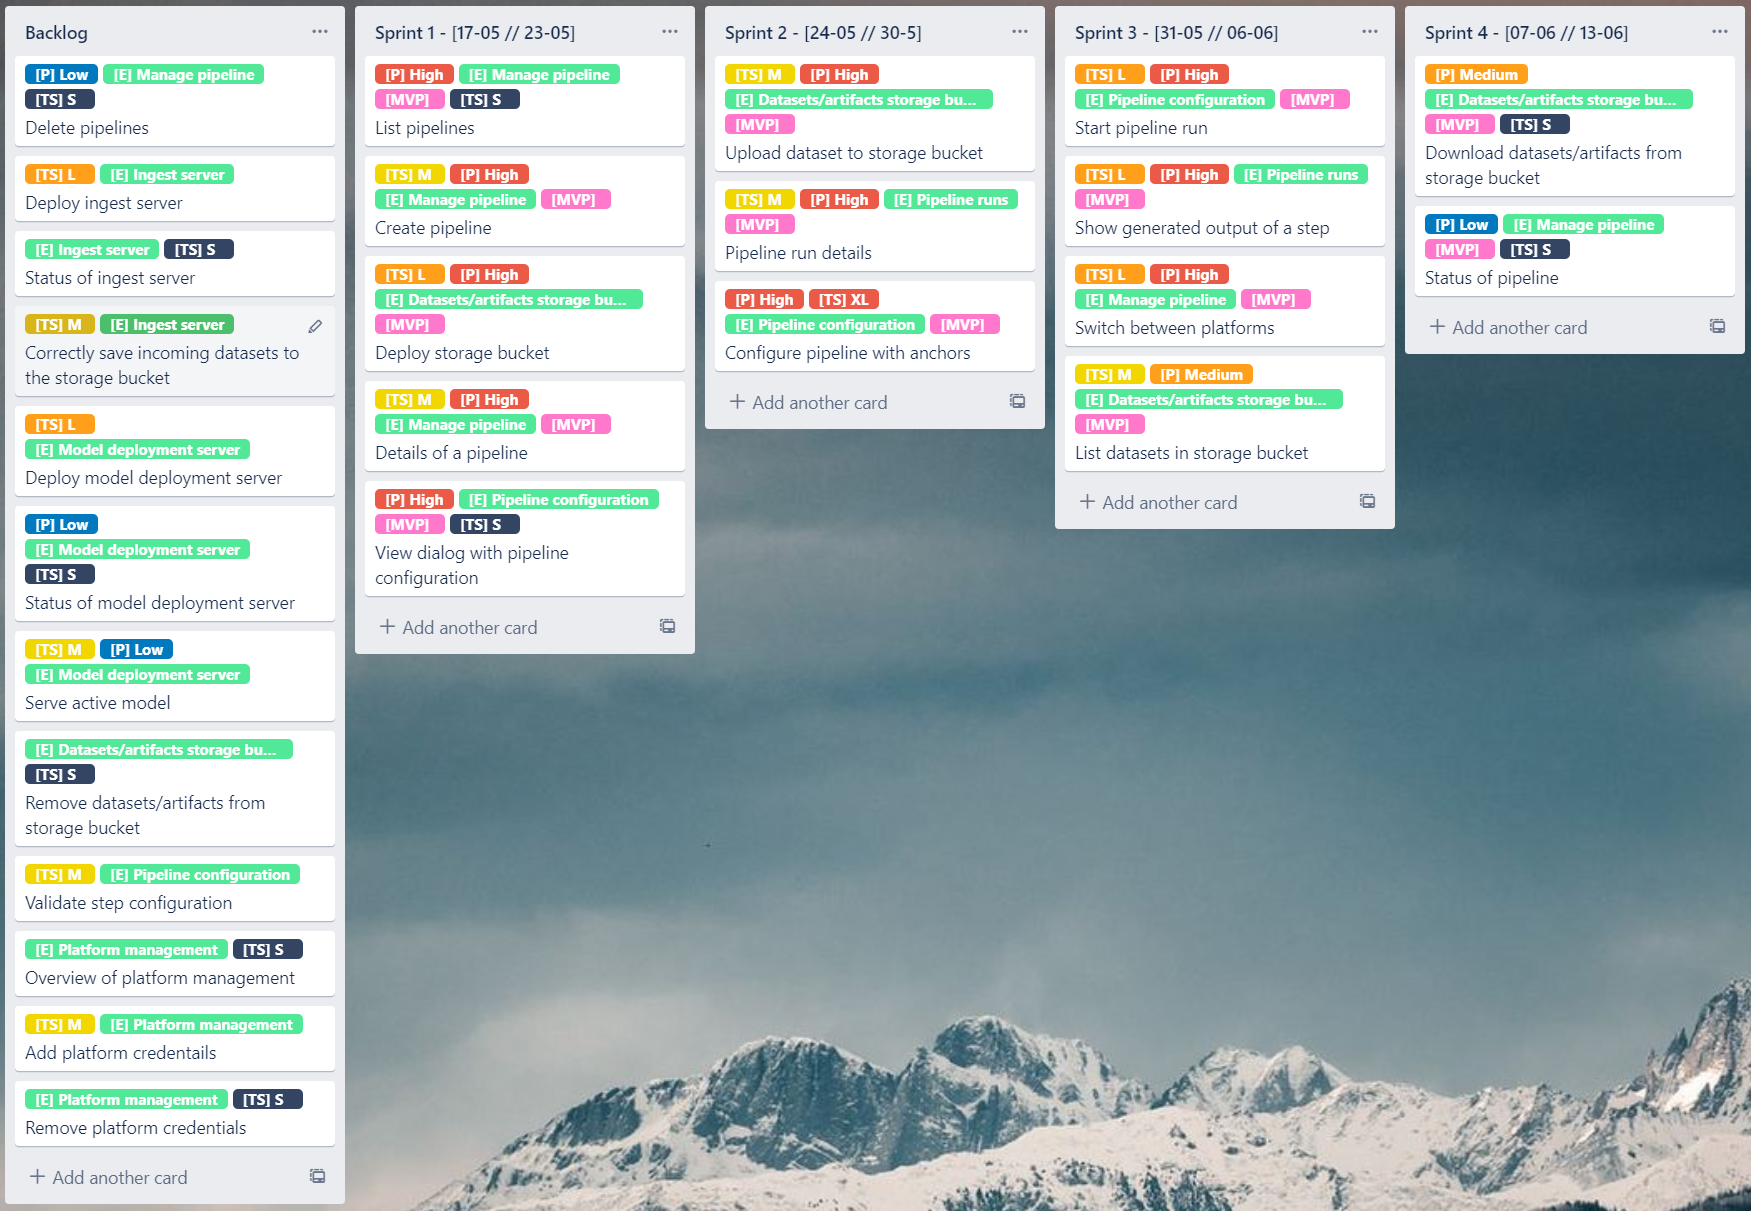
\includegraphics[width=0.99\textwidth]{chapter-7/trello-w1-start.png}
  \caption{Sprint 1.}
  \label{fig:ch7-trello-w1-start}
\end{figure}

In het ontwikkelproces is na elke sprint het scrum bord opnieuw bekeken om te reflecteren op de afgelopen sprint en de komende sprints opnieuw in te plannen als dit nodig was. In de bijlage is te zien hoe elke sprint is begonnen en geëindigd ([BIJLAGE LINK]). Nu de tickets aangemaakt zijn en de \acrshort{mvp} is vastgesteld, kan de mock up gemaakt worden.

\section{Mock up van de proof of concept}\label{sec:ch7-mock-up-van-de-proof-of-concept}
De mock up is bedoeld om te laten zien hoe de frontend van de PoC eruit gaat zien. Dit geeft ook de kans om te controleren of de \acrfull{ui} logisch in elkaar zit. Om de mock up te ontwerpen is gebruik gemaakt van Adobe XD \cite{adobe-xd}. De mock up bevat alleen functionaliteiten die \acrshort{mvp} zijn. 

Een pipeline wordt aangemaakt door het invullen van de naam en project ([BIJLAGE LINK]). Na het aanmaken van een pipeline kan erop geklikt worden. In \autoref{fig:ch7-mockup-mvp-pipeline-details} is de mock up van de details van een pipeline te zien. Op deze pagina is de status van de pipeline, configuration, dataset/artifacts en runs te zien.

\begin{figure}[hbt!]
  \centering
  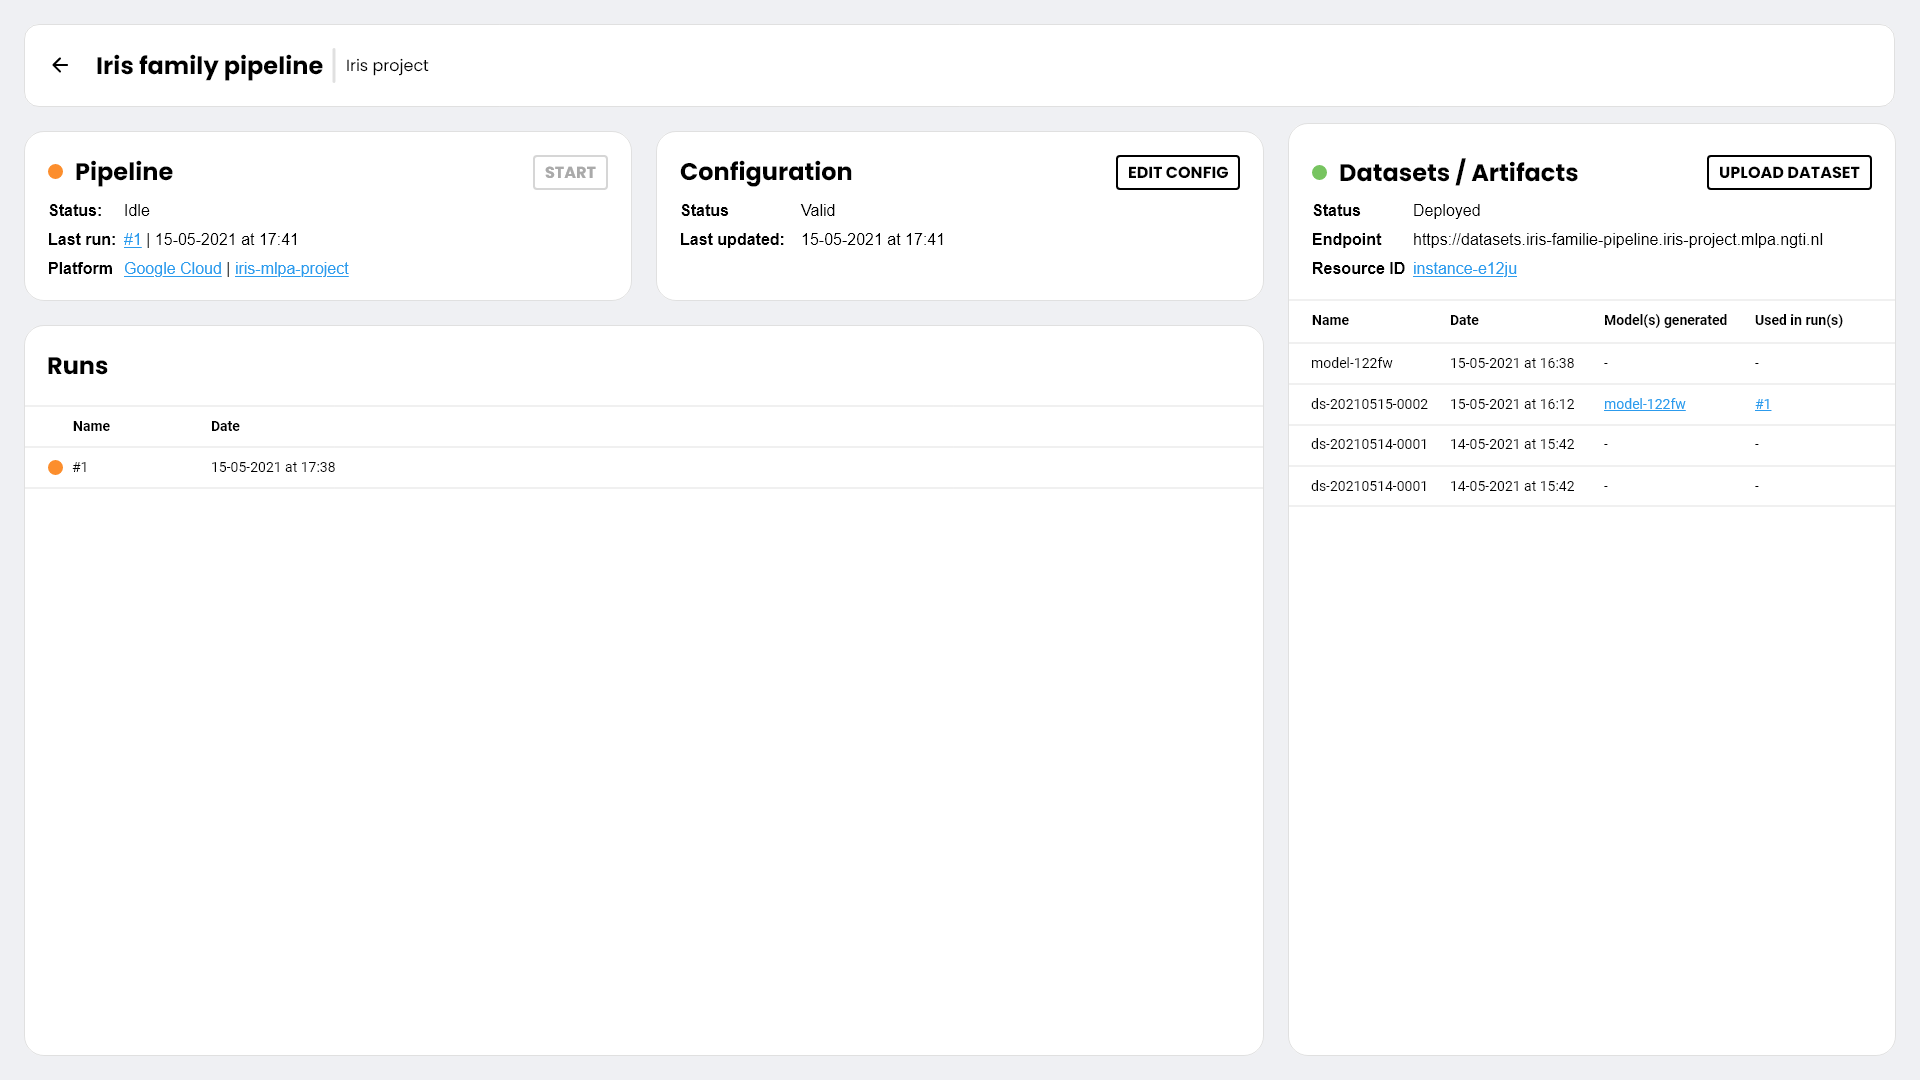
\includegraphics[width=0.99\textwidth]{chapter-7/[mvp]-pipeline-details.png}
  \caption{Mock up van de pipeline details pagina.}
  \label{fig:ch7-mockup-mvp-pipeline-details}
\end{figure}

De configuration is een Python script dat door de developer is gedefinieerd. De script wordt uitgevoerd als de pipeline wordt gestart. In de datasets/artifacts sectie kan de developer datasets en artefacts up- en downloaden. Als laatste kan de developer de status van de pipeline en run zien. Een run is een individuele run als een pipeline wordt gestart. Mock ups van andere gedeeltes van de PoC is te vinden in [BIJLAGE LINK]. Nu het voorwerk is gedaan, kan code voor de PoC geschreven worden.

\section{De proof of concept}\label{sec:ch7-de-proof-of-concept}
In \autoref{sec:ch6-architecturaal-ontwerp} is kort uitgelegd dat de backend gebouwd wordt met Node.js en Express en de frontend met React.js en TypeScript. Voor de PoC is een GitHub repository aangemaakt waarin de front- en backend geïnitialiseerd is met behulp van de documentatie van de frameworks. In de volgende koppen wordt in een logische volgorde door de applicatie gelopen waarbij uitleg over de werking wordt gegeven met screenshots van de \acrshort{ui} en code als ondersteuning.

\subsection{Aanmaken van pipelines}\label{subsec:ch7-aanmaken-van-pipelines}
Om te beginnen moet een pipeline aangemaakt kunnen worden. In de frontend gaat dit met een dialoog (\autoref{fig:ch7-create-pipeline-dialog}). Hierin kan de naam, project en cloud platform aangegeven worden.

\begin{figure}[hbt!]
  \centering
  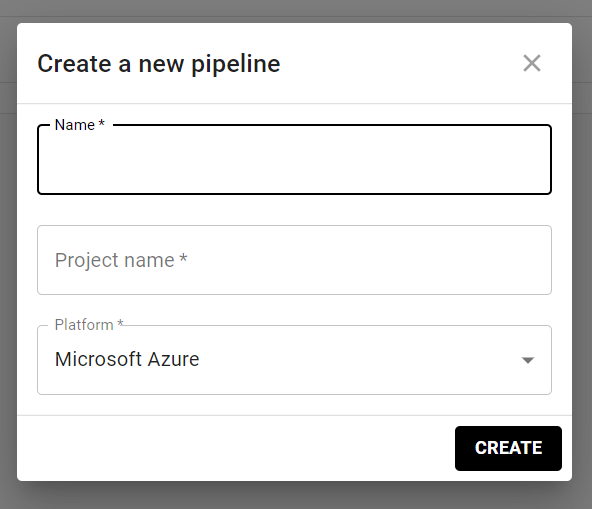
\includegraphics[width=0.5\textwidth]{chapter-7/poc-create-pipeline-dialog.png}
  \caption{Aanmaak dialoog van een pipeline.}
  \label{fig:ch7-create-pipeline-dialog}
\end{figure}

Zodra de developer klikt op de \textbf{Create} knop, wordt een request verstuurt van de frontend naar de backend. De backend stuurt de request naar een service dat ervoor zorgt dat de juiste acties uitgevoerd wordt. De service in \autoref{fig:ch7-create-pipeline-service} controleert welk platform er gespecificeerd is en spreekt de relevante functie aan. Als het platform bijvoorbeeld Google Cloud is, wordt de functie \(gc\_createBucket()\) op lijn 6 aangeroepen.

\begin{figure}[hbt!]
  \centering
  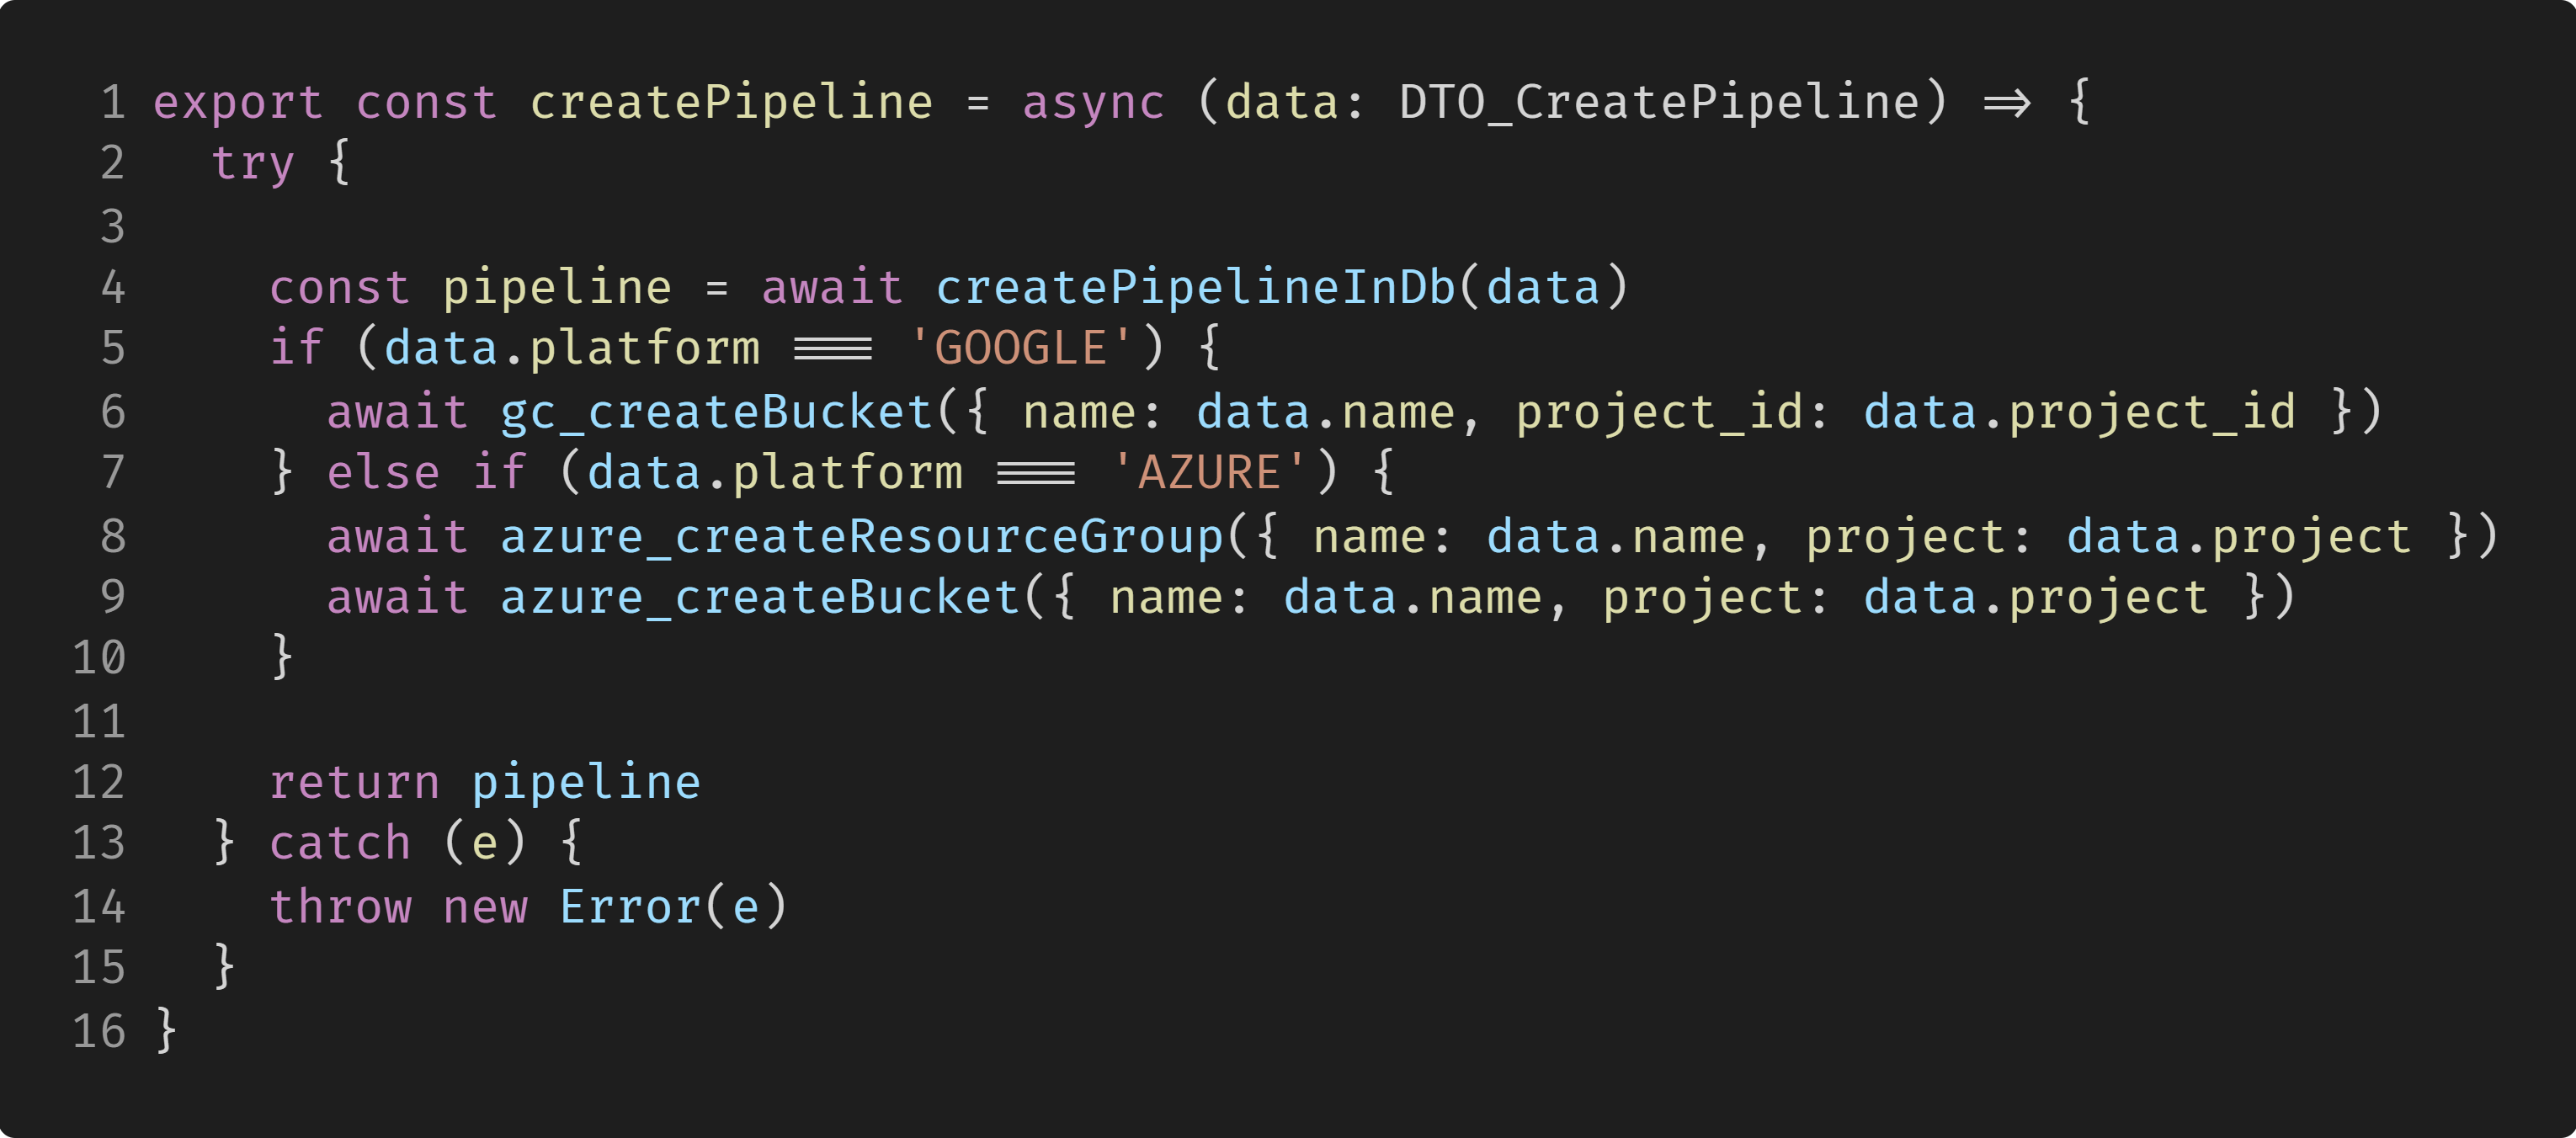
\includegraphics[width=0.85\textwidth]{chapter-7/poc-create-pipeline-service.png}
  \caption{Service om een pipeline aan te maken.}
  \label{fig:ch7-create-pipeline-service}
\end{figure}

Om een pipeline in Google Cloud aan te maken hoeft alleen een storage bucket aangemaakt te worden. De functie die deze actie uitvoert is te zien in \autoref{fig:ch7-create-pipeline-google-cloud}. De bucket heeft een naam nodig en de locatie. Op lijn 5 van \autoref{fig:ch7-create-pipeline-google-cloud} is \textbf{EUROPE-WEST4} gespecificeerd. Dit is een locatie in Nederland.

\begin{figure}[hbt!]
  \centering
  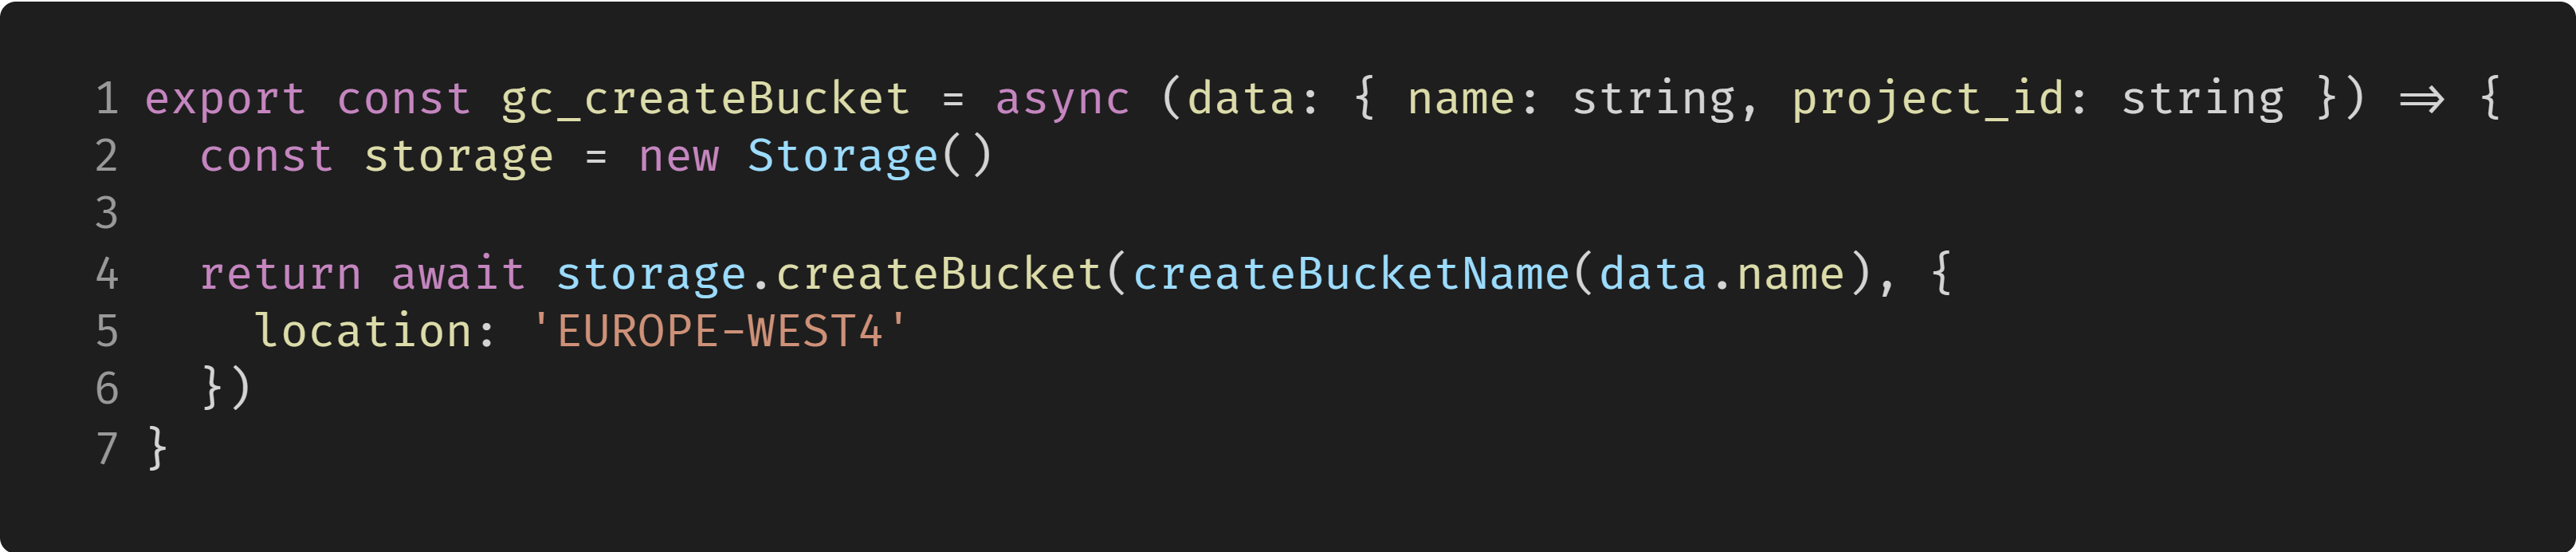
\includegraphics[width=0.9\textwidth]{chapter-7/poc-create-pipeline-google-cloud.png}
  \caption{Functie om een storage bucket aan te maken in Google Cloud.}
  \label{fig:ch7-create-pipeline-google-cloud}
\end{figure}

\newpage

Naast het aanmaken van de storage bucket in Google Cloud wordt de details van de pipeline opgeslagen in de PostgreSQL database (\autoref{fig:ch7-create-pipeline-service}, lijn 4). Na het aanmaken van een pipeline kan een dataset geüpload worden.

\subsection{Datasets uploaden}\label{subsec:ch7-datasets-uploaden}
Tijdens het aanmaken van de pipeline is een opslaglocatie in de cloud platform aangemaakt. In details weergave van een pipeline is een sectie weergegeven zoals in \autoref{fig:ch7-poc-upload-dataset} waar de developer datasets kan uploaden. Na het uploading krijgt de developer een confirmatie te zien en wordt de lijst met bestaande datasets en artefacts ververst.

\begin{figure}[hbt!]
  \centering
  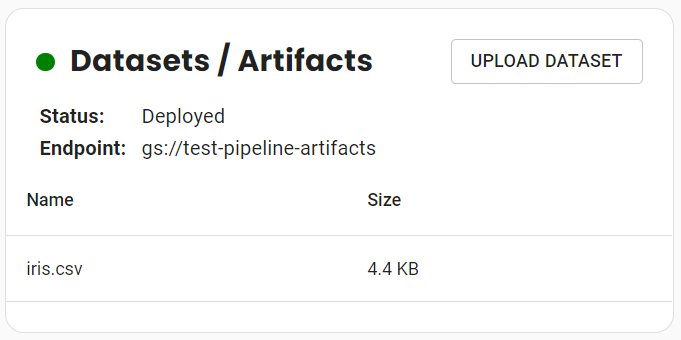
\includegraphics[width=0.9\textwidth]{chapter-7/poc-upload-dataset.png}
  \caption{Status en upload-mogelijkheid van datasets en artefacts in de details pagina van een pipeline.}
  \label{fig:ch7-poc-upload-dataset}
\end{figure}

De code in de backend voor het uploaden is vergelijkbaar met de code in \autoref{fig:ch7-create-pipeline-service} en \autoref{fig:ch7-create-pipeline-google-cloud}. In \autoref{fig:ch7-poc-upload-dataset-service} is de service te zien dat wordt wordt gebruikt als de developer een dataset upload in de frontend. De service selecteert de juiste functie om de dataset te uploaden om basis van het gekozen platform.

\newpage

\begin{figure}[hbt!]
  \centering
  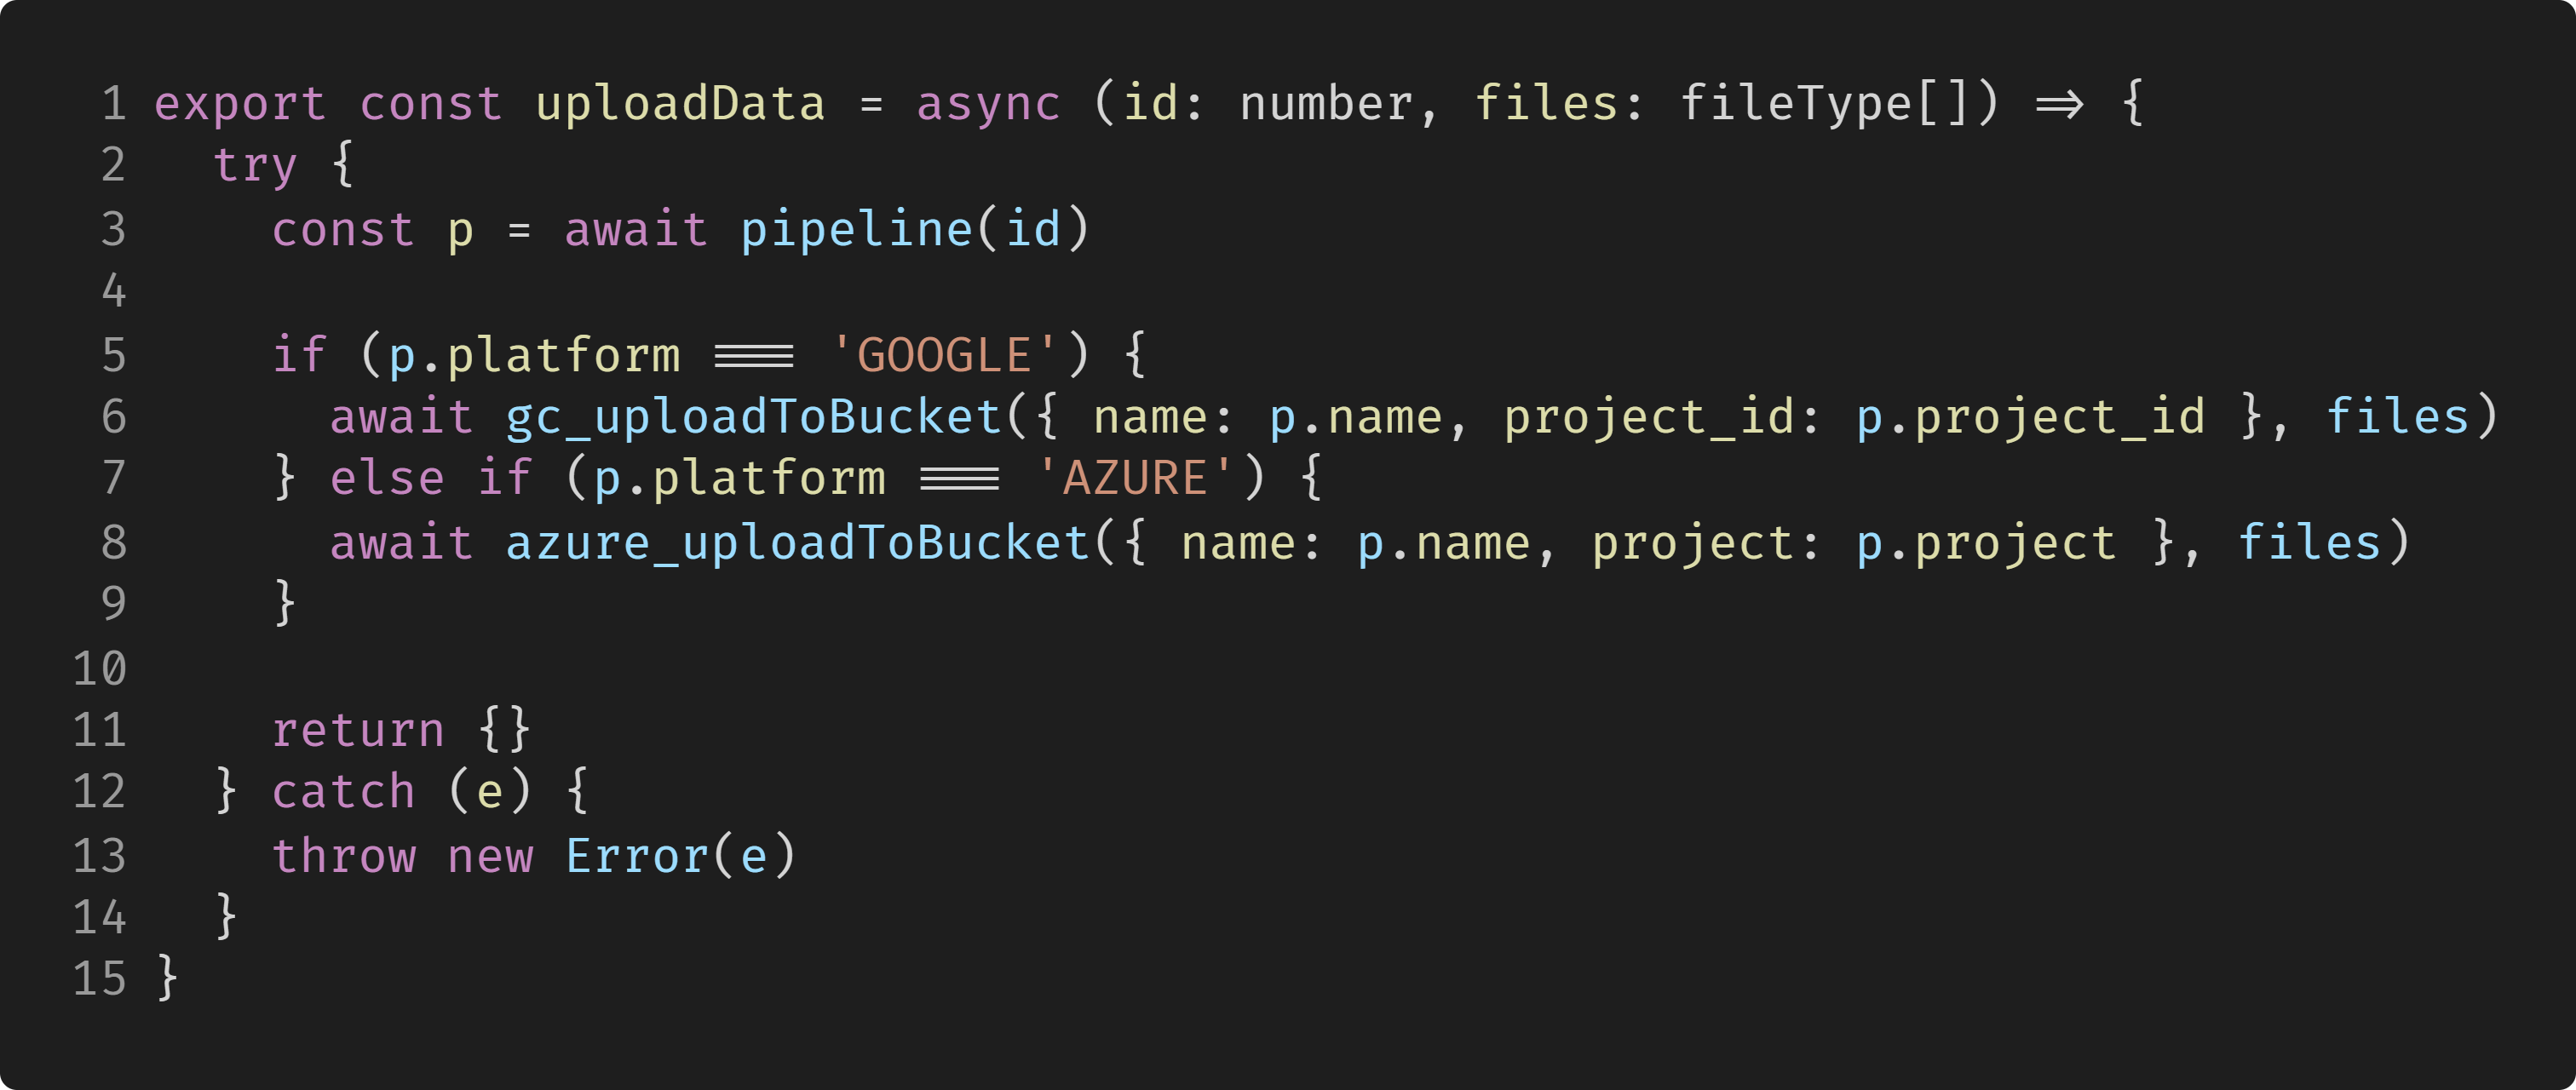
\includegraphics[width=0.8\textwidth]{chapter-7/poc-upload-dataset-service.png}
  \caption{Service om datasets te uploaden naar een opslaglocatie binnen een cloud platform.}
  \label{fig:ch7-poc-upload-dataset-service}
\end{figure}

\begin{figure}[hbt!]
  \centering
  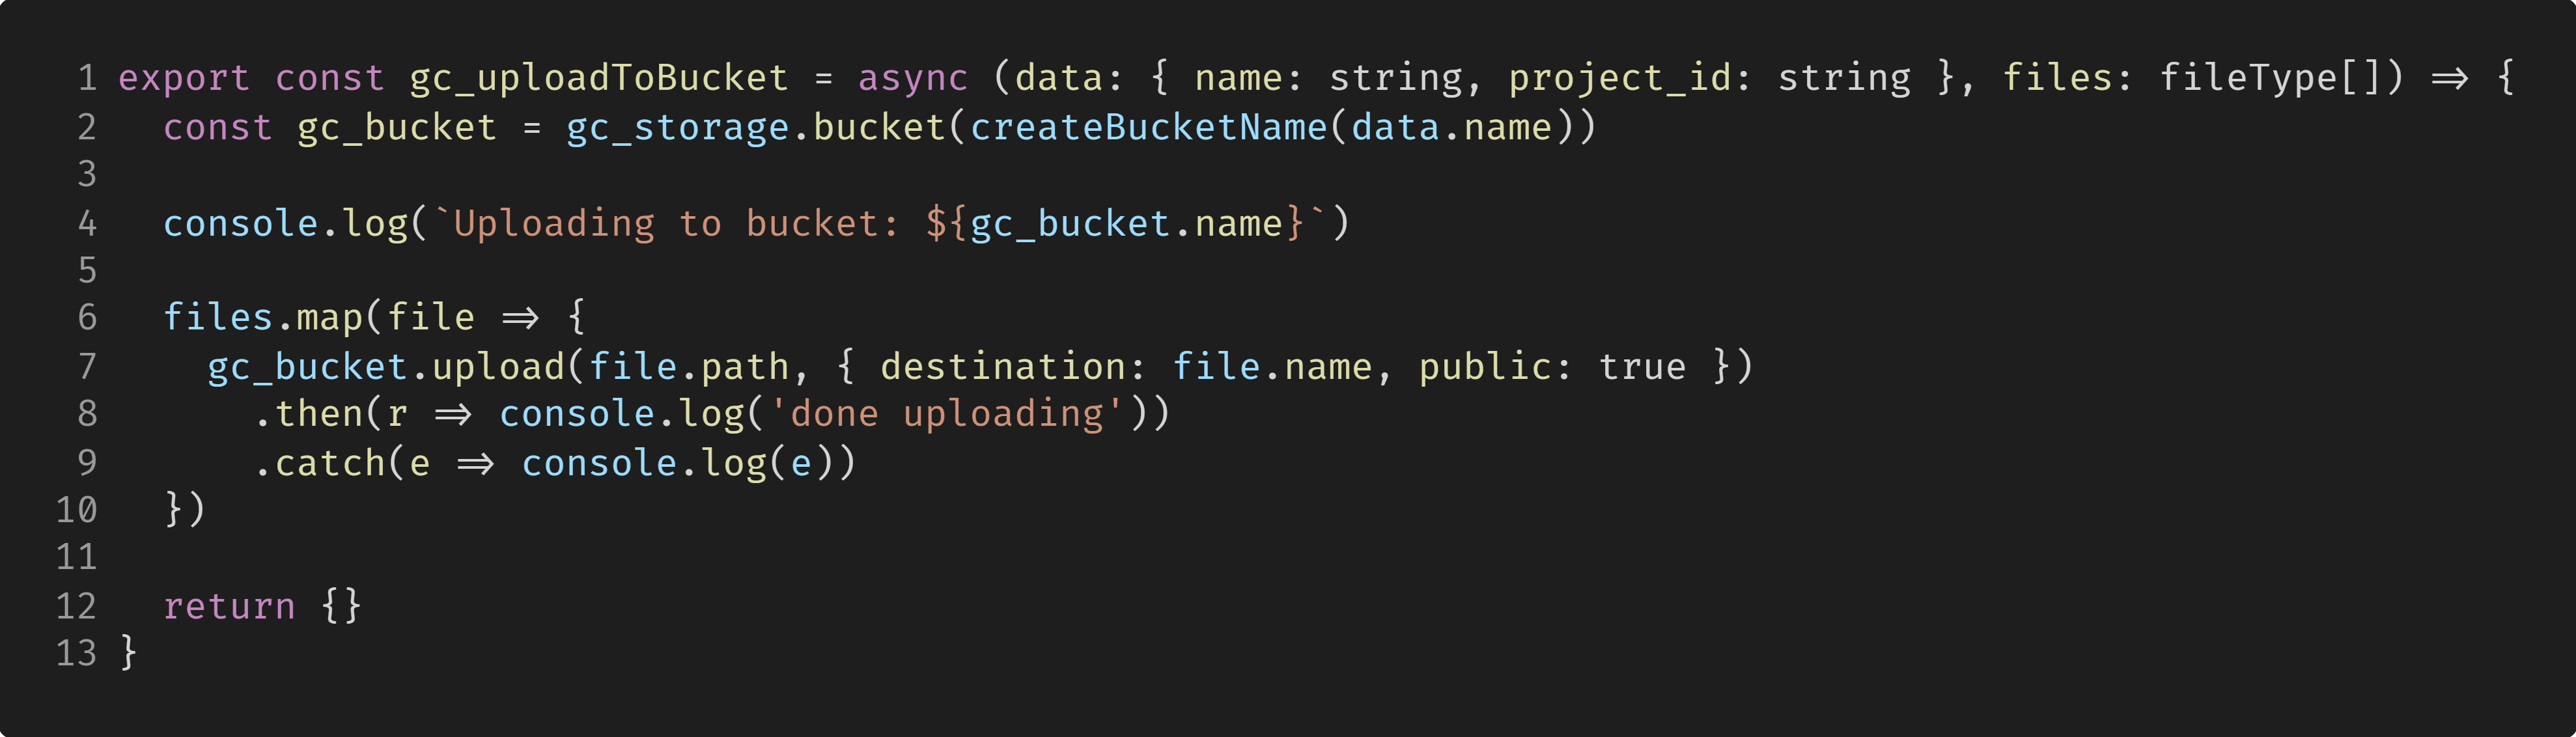
\includegraphics[width=0.9\textwidth]{chapter-7/poc-upload-dataset-google-cloud.png}
  \caption{Functie om datasets te uploaden naar een storage bucket in Google Cloud.}
  \label{fig:ch7-poc-upload-dataset-google-cloud}
\end{figure}

De backend maakt een instantie van de bucket in \autoref{fig:ch7-poc-upload-dataset-google-cloud} op lijn 2 en voert de \(upload()\) functie uit op lijn 7. De geüploade datasets zijn vervolgens beschikbaar om te gebruiken in de configuratie van de pipeline.

\newpage

\subsection{Configuratie definiëren}\label{subsec:ch7-configuratie-definieren}
Het laatste wat de developer moet doen om de pipeline te starten is het opgeven van de configuratie. Zoals aangegeven in \autoref{sec:ch7-mock-up-van-de-proof-of-concept} is de configuratie een Python bestand dat uitgevoerd wordt als de pipeline gestart wordt. In de PoC is de configuratie bewerkbaar door middel van een dialoog (\autoref{fig:ch7-poc-configuration-dialog}) met rechts een lijst van de datasets. De standaard configuratie dient als startpunt voor de developer. Een link naar de dataset kan gekopieerd worden door op een dataset te klikken.

\begin{figure}[hbt!]
  \centering
  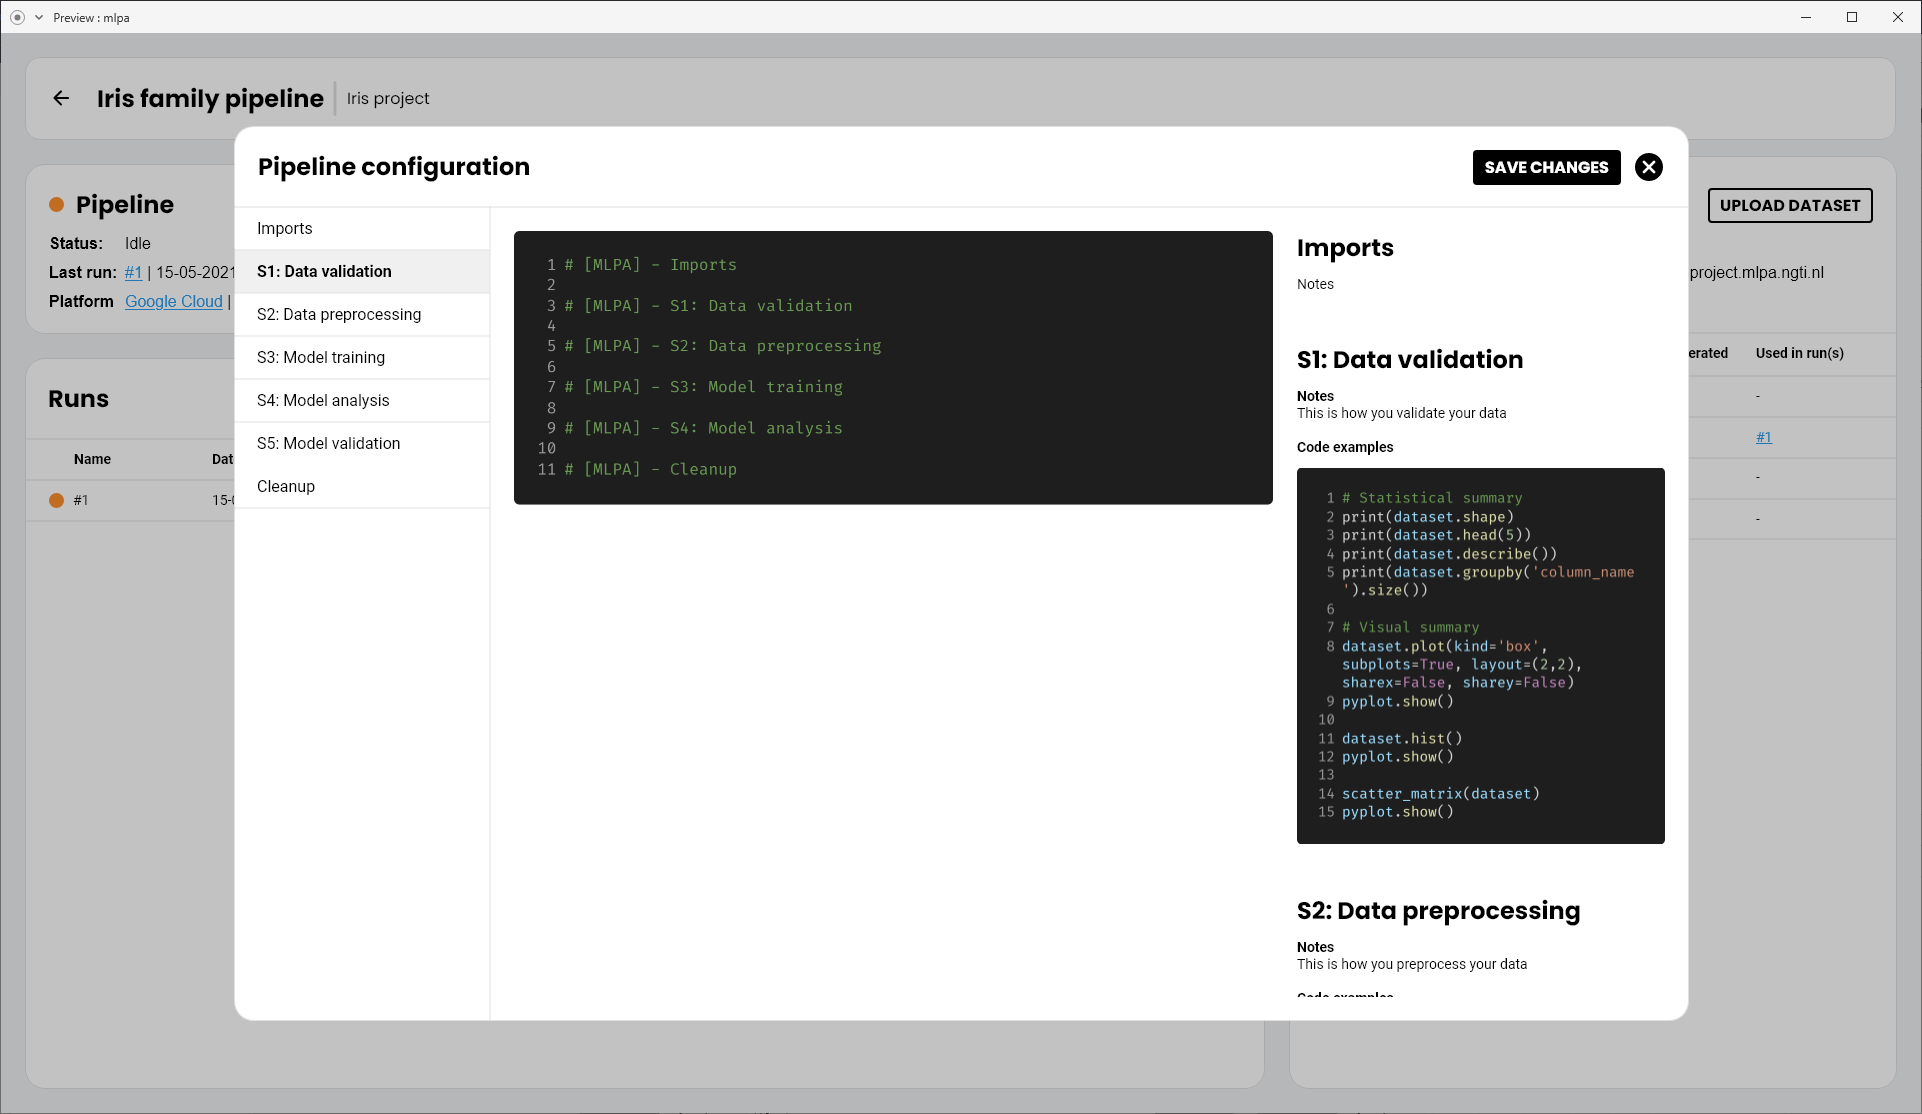
\includegraphics[width=0.9\textwidth]{chapter-7/poc-configuration-dialog.png}
  \caption{Configuratie dialoog van een pipeline.}
  \label{fig:ch7-poc-configuration-dialog}
\end{figure}

Zodra de developer op \textbf{SAVE} klikt, wordt een request gedaan naar de backend om de configuratie op te slaan. De code om de configuratie op te slaan is te zien in \autoref{fig:ch7-poc-configuration-commit-db}. Hier wordt een nieuwe configuratie aangemaakt en gelinkt aan de pipeline.

\begin{figure}[hbt!]
  \centering
  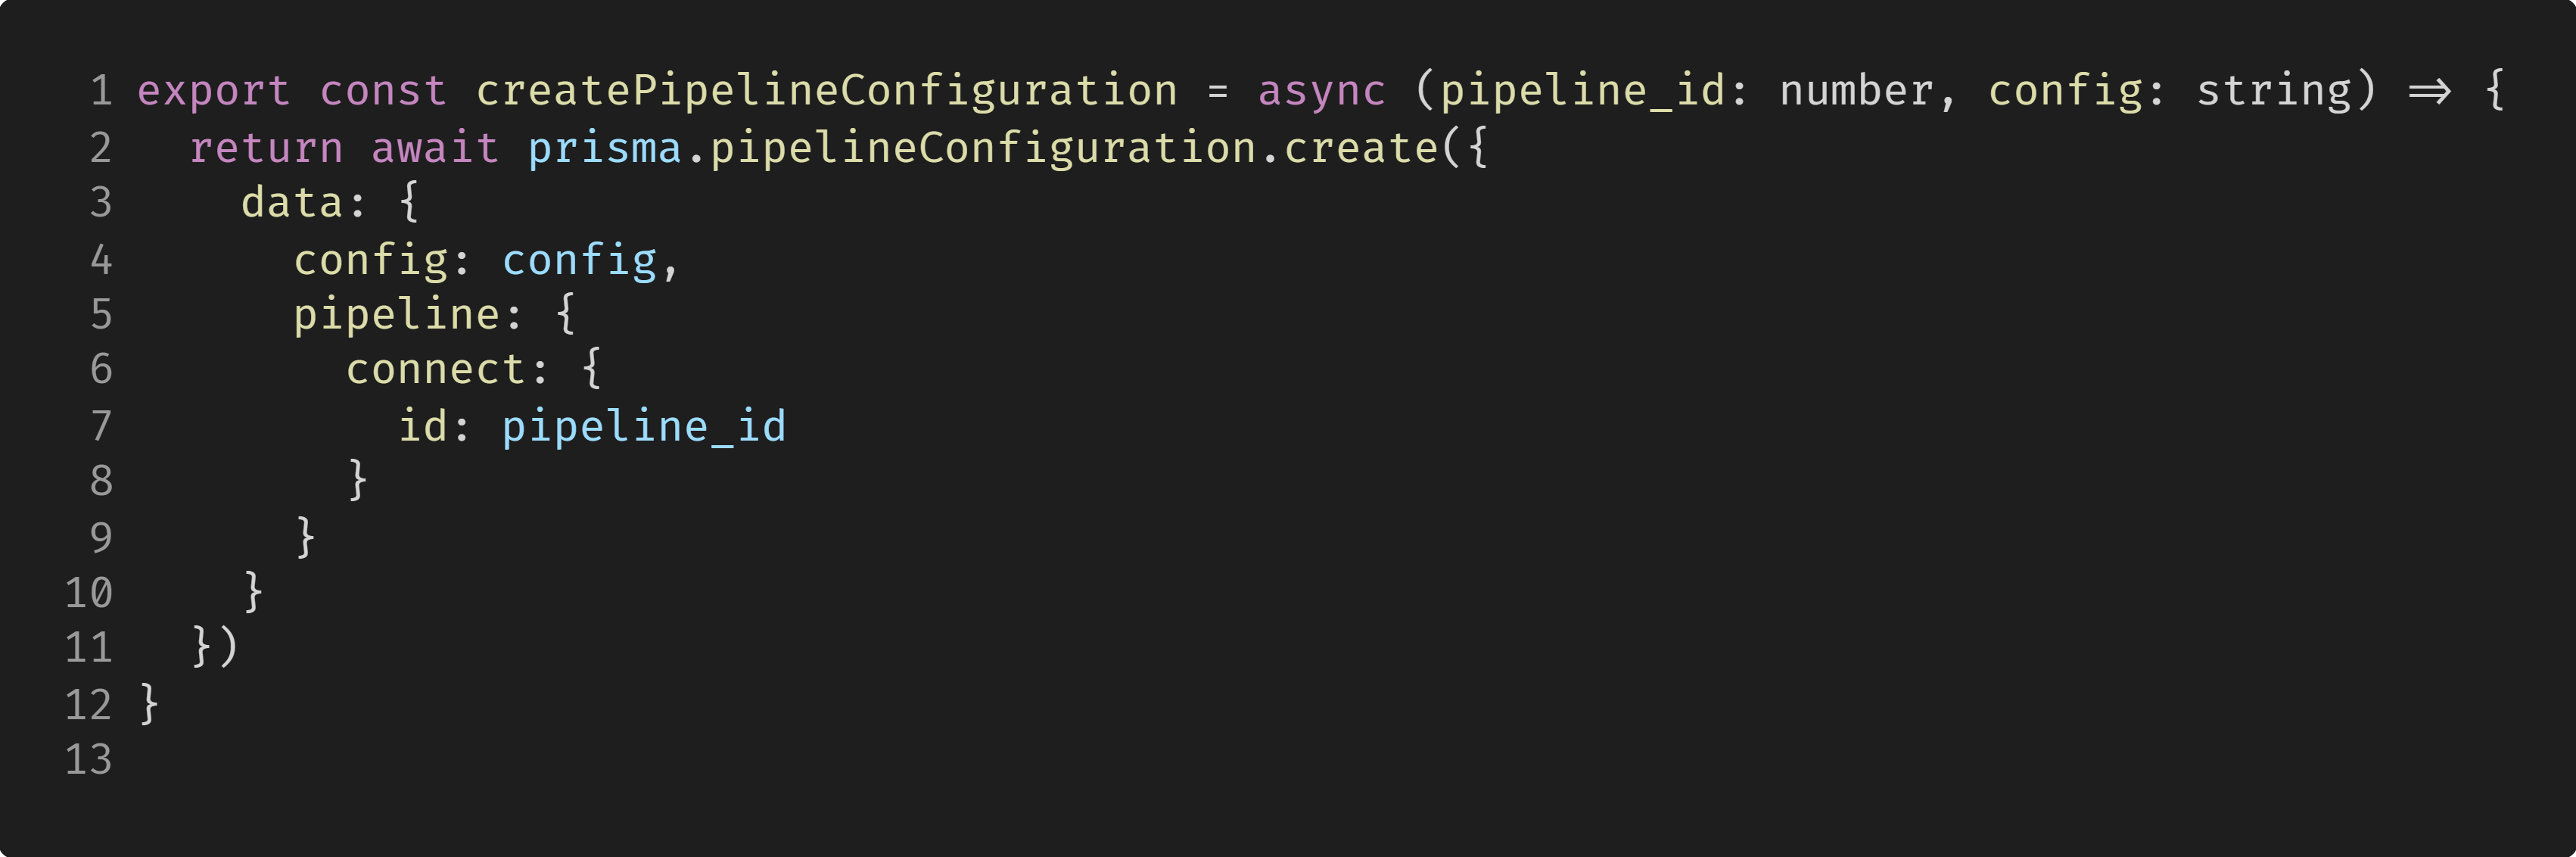
\includegraphics[width=0.85\textwidth]{chapter-7/poc-configuration-commit-db.png}
  \caption{Code om de configuratie op te slaan in de database.}
  \label{fig:ch7-poc-configuration-commit-db}
\end{figure}

Het is mogelijk om code te schrijven in andere talen dan Python om modellen te trainen. Om de complexiteit en scope klein en realistisch te houden is er gekozen voor Python. De taal is een van de populairste talen \cite{stack-overflow-survey-2020-loved-dreaded-framework-libraries-tools}. Daarnaast heeft Python een complete set van libraries om data te transformeren, plotten in diagrammen en modellen te trainen \cite{python-libraries}. Nu de configuratie is opgeslagen zijn alle benodigdheden beschikbaar om de pipeline te starten. 

\subsection{Pipeline starten}\label{subsec:ch7-pipeline-starten}


\subsection{Model downloaden}\label{subsec:ch7-model-downloaden}

\section{Kwaliteit van de code}\label{sec:ch7-kwaliteit-van-de-code}


% ---

\section{Conclusie}\label{sec:ch7-conclusie}


\section{Advies}\label{sec:ch7-advies}
